%
% maxwell.tex -- Bild zum Thema Optische Fouriertransformation <opt>
%
% (c) 2023 Marco Niederberger, Yanick Schoch; OST Ostschweizer Fachhochschule
%

\documentclass[tikz]{standalone}
\usepackage{tikz,tikz-3dplot}
% \usepackage{amsmath}
% \usepackage{txfonts}
\usepackage{pgfplots}

% \pgfplotsset{compat=1.16}
\def\skala{1}

%
% opt_common.tex -- Commands and color definition for the paper <opt>
%
% (c) 2023 Marco Niederberger, Yanick Schoch; OST Ostschweizer Fachhochschule
%

%%% NEW COMMANDS %%%

% Lense (x, height, curvature)
\newcommand{\lense}[3]{
    \def\curvature{0.2}
    \path[fill=glass, draw=black, line width = 0.6, opacity=0.8] (#1,-#2) .. controls (#1 - #3,0) .. (#1,#2) .. controls (#1 + #3,0) .. (#1,-#2);
}

% Dimension arrow (xStart, xEnd, yHeight, text)
\newcommand{\optMeasurement}[4]{%
    \draw[<->] (#1, #3)--(#2, #3) node[above,midway] {#4};
}

% Annotated point
\newcommand{\point}[3]{
    \draw[fill=black] (#1) circle (1pt) node[#3] {#2};
}

%%% COLORS %%%

% Define Color
\definecolor{glass}{cmyk}{0.2,0,0,0}
\colorlet{optBlue}{blue!70!black}
\colorlet{optRed}{red!90!black}
\colorlet{optGreen}{green!50!black}

%%% STYLES %%%

% Laser rays
\tikzset{red ray/.style = {optRed, line width = 0.6}}
\tikzset{ray arrow/.style = {red ray, postaction=decorate,decoration={markings,mark=at position 0.52 with \arrow{stealth}}}}


% \usetikzlibrary{arrows,intersections,math}
\usetikzlibrary{decorations.markings, } %calc

\begin{document}
% \tdplotsetmaincoords{70}{145}
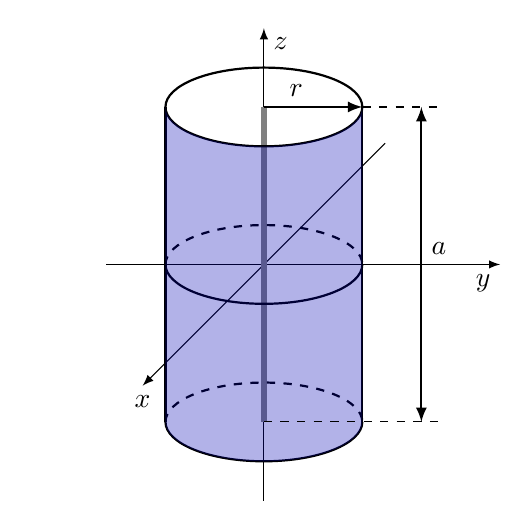
\begin{tikzpicture}[>=latex,thick,scale=\skala] %tdplot_main_coords
    \draw[draw=none](-3,0)--(3,0);

    % Coordinate
    \coordinate (O) at (0,0,0);
    \draw[->, thin] (-2,0,0) -- (3,0,0) node[anchor=north east]{$y$};
    \draw[->, thin] (0,-3,0) -- (0,3,0) node[anchor=north west]{$z$};
    \draw[->, thin] (0,0,-4) -- (0,0,4) node[anchor=north]{$x$};

    % Charge
    \draw[line width=2, gray] (0,-2,0) -- (0,2,0);

    % Cylinder shape
    \draw (0,2,0) ellipse (1.25 and 0.5);
    \draw (-1.25,2,0) -- (-1.25,-2,0);
    \draw (1.25,2,0) -- (1.25,-2,0);  
    \draw (-1.25,0,0) arc (180:360:1.25 and 0.5);
    \draw [dashed] (-1.25,0,0) arc (180:360:1.25 and -0.5);
    \draw (-1.25,-2,0) arc (180:360:1.25 and 0.5);
    \draw [dashed] (-1.25,-2, 0) arc (180:360:1.25 and -0.5);
    \fill [optBlue,opacity=0.3] (-1.25,2,0) -- (-1.25,-2,0) arc (180:360:1.25 and 0.5) -- (1.25,2,0) arc (0:180:1.25 and -0.5);

    % Measurement
    \draw[->] (0,2,0) -- (1.25,2,0) node[anchor=south east, midway]{$r$};
    \draw[<->] (2,-2,0) -- (2,2,0) node[anchor=south west, midway]{$a$};
    \draw[-,thin, dashed] (1.25,2,0)--(2.3,2,0);
    \draw[-,thin, dashed] (0,-2,0)--(2.3,-2,0);
\end{tikzpicture}
\end{document}

